\documentclass{article}
\usepackage{amsmath} %This allows me to use the align functionality.
                     %If you find yourself trying to replicate
                     %something you found online, ensure you're
                     %loading the necessary packages!
\usepackage{amsfonts}%Math font
\usepackage{graphicx}%For including graphics
\usepackage{hyperref}%For Hyperlinks
\usepackage{listings}
\lstset{
    numbers=left,
    backgroundcolor = \color{lightgray},
    breaklines=true,
    tabsize=2,
    basicstyle=\ttfamily,
    literate={\ \ }{{\ }}1
}
\usepackage{graphicx}
\usepackage{fancyvrb}
\usepackage{natbib}        %For the bibliography
\bibliographystyle{apalike}%For the bibliography
\usepackage[margin=1.0in]{geometry}
\usepackage{float}
\usepackage{tikz}
\usetikzlibrary{trees}
\begin{document}
%set the size of the graphs to fit nicely on a 8.5x11 sheet
\noindent \textbf{Caio Brighenti }\\
\noindent \textbf{COSC 302 - Analysis of Algorithms -- Spring 2019}\\%\\ gives you a new line
\noindent \textbf{Assignment 3}\vspace{1em}\\
\begin{enumerate}
	\item Maximum subarray
	\\ Our algorithm, in pseudocode, is as follows.
	\begin{lstlisting}
maxSubarray(array A){
		
	// keep track of max		
	max = 0
	// maximum subarray ending at A[j]
	currmax = 0
		
	for (i in A){
		// add current element
		currmax += A[i]
		
		// if subarray goes under 0, start new subarray
		currmax = max(currmax,0)
		
		if (currmax > max)
			max = currmax
		
	}				
	return max
}
	\end{lstlisting}
	This algorithm runs in linear time, as it visits each element in the array $A$ once. Next, we briefly explain the algorithm's functionality.
	\\ \textbf{Explanation}
	\\The algorithm consists of two persistent variables, and one loop. At all points, it keeps track of two sub array values: an overall maximum, stored in the variable max, and the maximum subarray ending at $A[j]$, stored in currmax. Both are initialized to 0, which is what we would expect for an empty array. Let us consider maintenance for each the variables throughout the loop, starting with currmax.
	\\ At any index $j$, the maximum subarray ending at $j$ must be equal to the maximum subarray ending at $A[j-1]$ plus the value at $A[j]$. In the case that $A[j]$ is positive, it is obvious that this continuous subarray will continue to grow. In the case that $A[j]$ is negative, the subarray will shrink, but if the subarray continues to be positive overall than it is still the greatest subarray up until $A[j]$, and is what is continued to $A[j+1]$. However, if $A[j]$ is sufficiently small, the subarray currmax may become smaller than 0, in which case we empty the subarray, as an empty subarray must a maximum with respect to a negative one. This is equivalent to choosing $A[j+1]$ as the new beginning of the subarray which will now be considered.
	\\ We have shown the algorithm appropriately calculates the largest subarray ending at each index $j$ in $A$. The algorithm will always set the variable max to be the largest of these subarrays. As a maximum subarray in $A$ must end at an index $j$, than the variable max will have the largest subarray in $A$, and thus the algorithm is correct.
\\ \textbf{Running time}
\\ The objective of this problem was not simply to provide a correct algorithm for the max-subarray problem, but to do so in linear time, non-recursively. Thus, we must show that this algorithm is both linear and non-recursive. Showing that it is non-recursive is trivial-- the algorithm makes no calls to itself and thus is clearly non-recursive. Next we show the running time.
\\ When called, the algorithm performs constant time operations in lines 4 and 6, and executes a loop in lines 8-18. We can see clearly that the contents of the loop also run i constant time, as there are simply the operations on lines 10, 13, 15, and 16. It is also clear the number of iterations of the loop depends on the size of $A$, which we call $n$, as it iterates through each item in the array. Thus our overall running time is $\Theta(1)+\Theta(n)\Theta(1)\in \Theta(n)$. Thus, the algorithm is  both linear and non-recursive.
\item \textbf{Reccurence relations}
	\begin{enumerate}
	\item Solve $T(n)=T(\frac{n}{2})+T(\frac{n}{4})+T(\frac{n}{8})+n$ using recursion tree and induction.
	\\ \\ \textbf{Recursion Tree:}
	\\ We proceed by recursion tree first by drawing the tree, though here we show only the first two levels.
\begin{center}
	\begin{tikzpicture}[level distance=1.5cm,
	  level 1/.style={sibling distance=3cm},
	  level 2/.style={sibling distance=1.5cm}]
	  \node {n}
	    child {node {$\frac{n}{2}$}
	    }
	    child {node {$\frac{n}{4}$}
	    }
	    child {node {$\frac{n}{8}$}
	    };
	\end{tikzpicture}
\end{center}
We can see that each level sums up to $\frac{7}{8}$ of the level before it, as each node separates into that ratio. This may seem an unfounded assumption, but is easy to show using basic multiplication properties. The second level is clearly $\frac{1}{2}+\frac{1}{4}+\frac{1}{8}=\frac{7}{8}$ of $n$, and thus we can see that each of the three children of a node sum up to $\frac{7}{8}$ of that node. Thus we can consider the third level as $\frac{7}{8}\frac{n}{2}+\frac{7}{8}\frac{n}{4}+\frac{7}{8}\frac{n}{8}=\frac{7}{8}(\frac{n}{2}+\frac{n}{4}+\frac{n}{8})=\frac{7}{8}(\frac{7}{8}n)$. This means that we can consider each level as $\frac{7}{8}$ of the previous level.
\\We might naively assume that each node performs work $n$, given the recurrence has a $n$ term in it. However, the problem becomes progressively smaller. Summing across each level, we instead have that each level performs work $(\frac{7}{8})^in$, where $i$ is the level. Thus, we can find the total work done by the algorithm by summing up each level. This sum takes the form $(\frac{7}{8})^0n + (\frac{7}{8})^1n + \cdots + (\frac{7}{8})^in$. This is a geometric series, therefore we can simplify it to $\frac{1}{1-\frac{7}{8}}n = 8n$ which is plainly in $O(n)$.
	\\ \\ \textbf{Induction:}
\\ We proceed by induction, using the guess of $O(n)$ from the recursion tree solution. Formally, we want to show that $T(\frac{n}{2})+T(\frac{n}{4})+T(\frac{n}{8})+n \leq c n$ for all $n \geq n_0$, where $c$ is a positive constant. 
\\ \textbf{Base case - n=8 :}
Let us treat $n=8$ as the base case and show that the claim holds. We assume that $T(n)=n$ for all $n<8$, as otherwise the recurrence would proceed to make calls with non-integer parameters. Let $c=2$. Using these values, we have:
\\ $T(8) = T(4)+T(2)+T(1)+8 = 4+2+1+8=15$
Thus we have that $T(8) \leq 2 8$, so the base case holds.
\\ \textbf{Inductive Hypothesis:} Assume the claim holds for all $m$ such that $n_o \leq m < n$. We show that this implies the claim is true for $n$.
\begin{align}
	T(n)&=T(\frac{n}{2})+T(\frac{n}{4})+T(\frac{n}{8})+n && \text{reccurence} \\
	&\leq \frac{2n}{2} + \frac{2n}{4} + \frac{2n}{8} + n && \text{inductive hypothesis} \\
	&\leq n(1+\frac{1}{2}+\frac{1}{4}+1) && \text{algebra} \\
	&\leq 2.75 n \leq cn && \text{algebra}
\end{align}
Thus, the claim must be true for all $n\geq n_0$ and the positive constant $c=2$. 
\item Solve $T(n)=5T(\frac{n}{5})+\frac{n}{\log n}$ using recursion and the iteration method.
\\ \\ \textbf{Recursion tree}
	\\ We proceed by recursion tree first by drawing the tree, though here we show only the first two levels.
\begin{center}
	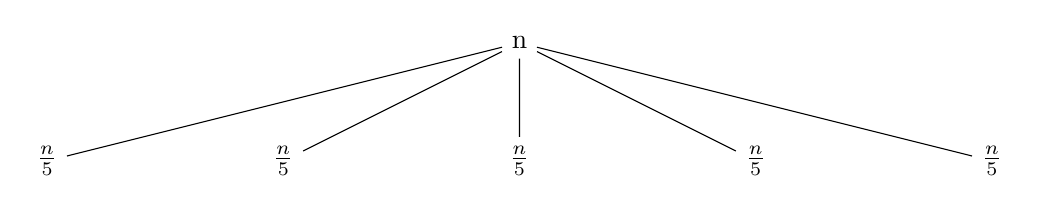
\begin{tikzpicture}[level distance=1.5cm,
	  level 1/.style={sibling distance=3cm},
	  level 2/.style={sibling distance=1.5cm}]
	  \node {n}
	    child {node {$\frac{n}{5}$}
	    }
	    child {node {$\frac{n}{5}$}
	    }
	    child {node {$\frac{n}{5}$}
	    }
	    child {node {$\frac{n}{5}$}
	    }
	    child {node {$\frac{n}{5}$}
	    };
	\end{tikzpicture}
\end{center}
Let $i$ be the last level in tree. As at each level $j$ each node is equal to $\frac{n}{5^j}$, then at the last level we have $\frac{n}{5^i}=1$. We can thus solve for $i=\log_5 n$, and we have that $n=5^i$. Both these facts will be useful to us.
\\ At each level $j$, each node does work $\frac{\frac{n}{5^j}}{\log \frac{n}{5^j}}$. As each level has $5^j$ nodes, then the total work per level is clearly $\frac{n}{\log \frac{n}{5^j}}$. Substituting, we have $\frac{5^i}{log5^{i-j}}$.
At the final level, the work per node will be $\Theta(1)$. Therefore, we solve for the total amount of work as follows. 
\begin{align}
T(n) &= 5^i + \sum_{j=0}^{i-1} \frac{5^i}{log_55^{i-j}} && \text{final level + other levels } \\
&= n + n \sum_{j=0}^{i-1} \frac{1}{i-j} && \text{$5^i=n$, $log_55^x=x$} \\
&= n + n \sum_{j=1}^{i} \frac{1}{j} && \text{harmonic series} \\
&= \Theta(n+n\log i) && \text{asymptotic nature of harmonic series} \\
&= \Theta(n+n\log \log n) && \text{i= logn}
\end{align}
Thus, we have that the recurrence relationship $T(n)=5T(\frac{n}{5})+\frac{n}{\log n}$ solves to $\Theta(n+n\log \log n)$.
\\ \\ \textbf{Iteration Method:}
\\ To solve this recurrence using the iteration method, we first have to calculate the total number of calls, then calculate the time per calls. Finally, we multiply the two together to obtain the total running time.
\\ \textbf{Number of calls}
\\ Let $j$ represent a level in the tree. At each level, there are $5^i$ recursive calls. Let $i$ be the last level. As each recursive call divides $n$ by 5, it must be that at the last level $\frac{n}{5^i}=1$. We can thus solve for $i=log_5n$. As $i$ is the last level, the total amount of levels must be $i+1$. 
\\ We can solve for the total number of calls by summing the number of calls per level. This is equal to the series $5^0+5^1+\cdots+ 5^i$, which simplifies to $5^{i+1}-1=5^{\log_5n+1}-1= 5^{\log_55n}-1= 5n-1\approx n$. We now find the time per call.
\\ \textbf{Time per call}
\\ We might naively assume that the time per call is simply $\frac{n}{\log n}$, as is the term in the recurrence. However, the problem gets smaller at each level $j$, making the actual time per call equal to $\frac{5^{i-j}}{\log 5^{i-j}}$. This presents a problem for us, as we cannot appropriately remove the $j$ term when multiplying by the number of calls and we are solving for a solution with respect to $n$. Therefore, we will compute the sum across all values of $j$ to obtain the total running time, and which we will then divide by the number of calls to compute the average running time per call. Thankfully, we have already computed this sum in the previous problem and know it to be $\in \Theta(n+n\log \log n)$. This is actually the answer we are looking for, so we have no need to divide and multiply again, but we do so nonetheless for clarity. As the total running time is $\in \Theta(n+n\log \log n)$, then the average running time per call must be $\in \Theta(\frac{n+n\log \log n}{n})=\Theta(1+\log \log n)$, as the total number of calls is $\Theta(n)$.
\\ \textbf{Overall running time}
\\ The overall running time is equal to the number of calls multiplied by the expected time per call. As the number of calls is $\in \Theta(n)$ and the time per call is $\in \Theta(1+\log \log n)$, the total running time must be $\Theta(n+n\log \log n)$.
	\item Using substitution method for the following recurrence prove that $T(n)\in O(n \log n)$ and $T(n) \in \Omega(n \log n)$ and conclude that $T(n)\in \Theta(n \log n)$.
	\\\\ We start by showing that $T(n)\in O(n \log n)$ using induction. We must show that $T(n-1)+\log n \leq c_2 n \log n$. We start with our base case.
	\\ \textbf{Base case: $n=1$, $c_2=3$}
	\\ We plug in $n$ and $c$ into the claim and obtain $T(1)=T(0)+\log 1= 0$. Next, we compute $c_2 n \log n = 3 \cdot 1 \cdot \log 1 = 0$, and as $0 \geq 0$, the base case holds. We proceed with our inductive hypothesis.
	\\ \textbf{Inductive Hypothesis}
	\\ For our inductive hypothesis, we assume that the claim holds for $c_2>3$ and for all $m$ such that $n_o \leq m < n$. We show that this implies the claim is true for $n$.
	\\\\ \emph{Notice 1:} for a sufficiently large $c_2$ and $n$, $(n-1)^{c_2}\geq n$. This is an intuitive claim, but we can confirm it by taking the limit of $\frac{(n-1)^{c^2}}{n}$, where $c^2$ is a positive constant greater than or equal to 2, which evaluates to $\infty$. 
	\begin{align}
	T(n) &= T(n-1)+\log n && \text{claim} \\
	& \leq c_2(n-1)\log (n-1)+\log n && \text{inductive hypothesis} \\
	&\leq c_2n\log(n-1)-c_2 \log (n-1) + \log n && \text{expand terms} \\
	&\leq c_2n\log(n-1)-\log((n-1)^{c_2})+\log n && \text{log rules} \\
	&\leq c_2n\log(n-1) && \text{$\log$ is monotonically increasing, notice 1} \\
	&\leq c_2n\log(n) && \text{$\log(n-1) < \log n$}
	\end{align}
Line 18 of the proof requires more clarity. As this is an inequality, we are free to make the right hand side larger by adding terms of removing negative terms. Based on notice 1, and on the fact that $\log$ is a monotonically increasing function, the negative $\log((n-1)^{c_2})$ term will outweigh the $\log n$ term, thus we can remove both terms. Thus we have that $T(n) \leq c_2n\log n$, and therefore that $T(n) \in O(n\log n)$. 
\\\\We also must show that $T(n) \in \Omega(n\log n)$. To do this we show that $c_1 n \log n \leq T(n)$. We start with our base case.
	\\ \textbf{Base case: $n=1$, $c_1=0.5$}
	\\ We plug in $n$ and $c$ into the claim and obtain $T(1)=T(0)+\log 1= 0$. Next, we compute $c_1 n \log n = 0.5 \cdot 1 \cdot \log 1 = 0$, and as $0 \geq 0$, the base case holds. We proceed with our inductive hypothesis.
\\ \textbf{Inductive Hypothesis}
\\ We assume that the claim holds for all $m$ such that $n_0 \leq m \leq n$ and for a positive constant $c_1$. We show that this implies the claim holds for $n$.
\\\\ \emph{Notice 2:} for a sufficiently small positive constant $c_1$ and for all $n>n_0$, we have $(n-1)^{c_1} < n$. The precise range for $c_1$ is $0 < c_1 < 1$, as it is clear that for any $c_1$ in this range, $x^{c_1} < x$, where $x$ is any positive number.
	\begin{align}
	T(n) &= T(n-1)+\log n && \text{claim} \\
	&\geq c_1(n-1)\log (n-1)+\log n && \text{inductive hypothesis} \\
	&\geq c_1n\log (n-1) - c_1\log (n-1) + \log n && \text{algebra} \\
	&\geq c_1n\log (n-1) && \text{notice 2, log is monotonically increasing}
	\end{align}
Line 19 of the proof requires more clarity. As this is an inequality, we are free to make the right side smaller by subtracting more terms. Based on notice 2, and on the fact that the log function is monotonically increasing, it must be that $\log n > c_1 \log (n-1)$. Thus, the first term outweighs the second and we can eliminate both, as the net result is positive and contributes to the size of the right hand side.
\\ We are left with $T(n) \leq c_1n \log(n-1)$, meaning we thus have $T(n) = \Omega(n\log(n-1)) \in \Omega(n\log n)$
\\ As we have shown that $T(n) \in O(n \log n)$ and $T(n) \in \Omega(n\log n)$, it follows that $T(n) \in \Theta(n\log n)$.
	\end{enumerate}
\item \textbf{Quick sort}
	\\ By combining the quick sort algorithm with the insertion sort algorithm, we will have an algorithm composed of two smaller pieces. To show the overall running time for this algorithm, we consider each section separately and then combine the two.
	\\ \\ \textbf{Quick sort:}
	\\ For simplicity, we consider quick sort with a balanced partition each time. Each level will thus divide $n$ by 2, until we reach the level such that $n$ goes to 1. By stopping when the subarrays at equal to $k$, however, we stop at the level $\frac{n}{k}$. Thus, the typical running time goes form $O(n\log n)$ to $O(n\log \frac{n}{k})$. This leaves $\frac{n}{k}$ arrays of length $k$ which must be sorted by insertion sort.
	\\ \\ \textbf{Insertion Sort:}
	\\ The running time of insertion sort is $O(n^2)$ in the worst and average case. We assume one of these two cases, as the best case is unreasonable in this case, given that it assumes the array is already sorted. Thus the total running time for sorting all unsorted arrays with insertion sort is $\frac{n}{k}O(k^2)$. Through algebra, this can be clearly simplified to $O(nk)$.
	\\ \\ \textbf{Overall running time:}
	\\ As we first sort most of the array using quick sort, and sort the remainder with insertion sort, the overall running time is equal to the sum of both pieces. Thus, the overall running time is $O(n\log \frac{n}{k}) + O(nk)= O(n\log \frac{n}{k} + nk)$. Next we consider how to choose a value $k$
	\\ \\ \textbf{Choosing K:}
	\\ It is plain to see that we need a value $k$ such that $ n\log n > n\log \frac{n}{k} + nk$. Let us thus solve for $k$ in this inequality.
	\begin{align}
	n \log n &> n \log \frac{n}{k} + nk  && \text{} \\
	\log n &> \log \frac{n}{k} + k && \text{divide both sides by $n$} \\
	\log n &> \log n - \log k + k && \text{log rules} \\
	\log k &> k && \text{subtract $\log n$, algebra}
	\end{align}
	This is clearly impossible, and would suggest no such $k$ exists. However, this is because we must consider the constant terms. We solve again, this time including the constant $c_1$ for quick sort and the constant $c_2$ for insertion sort.
		\begin{align}
	c_1 n \log n &>c_1 n \log \frac{n}{k} + c_2 nk  && \text{} \\
	c_1 \log n &> c_1 \log \frac{n}{k} + c_2 k && \text{divide both sides by $n$} \\
	c_1 \log n &> c_1 \log n - c_1\log k + c_2 k && \text{log rules} \\
	\log k &> \frac{c2}{c1} k && \text{subtract $c_1 \log n$, algebra}
	\end{align}
	Thus, using the constant terms from quick sort and insertion sort we would be able to locate a value of $k$ such that this combination of algorithm works more efficiently than simply using quick sort. In practice, we might also find such a $k$ more easily through statistical simulation. That is, we might randomly generate high volumes of arrays to be sorted, and experiment with different values of $k$ to experimentally determine a value that minimizes the runtime.
\item \textbf{Heap data structure}
	\begin{enumerate}
		\item How would you represent a $d$-ary heap in an array?
\\\\ We consider an array representation indexed by 1, such that the root of the heap is at $A[1]$. As any node will have $d$ children, the children of the root must be in the range $A[2]$ to (inclusive) $A[d+1]$. Each of these $d$ children will have $d$ children themselves, giving the third level $d^2$ children, which will be in the range $A[d+2]$ through $d^2+d+1$. This pattern continues (the next level will have $d^3$ items, the next $d^4$, and so forth.)
\\ We also need a system to calculate the parent and children of a node using its index $i$. Suppose that we can calculate the parent of a node $i$ with $\lfloor  \frac{i-2}{d+1} \rfloor$ and the children by $d(i-1)+j+1$, where $j$ represents the $j-th$ child of $i$ in the range $1\leq j \leq d$. We can see that this procedure works by choosing any appropriate $i$, $j$, and $d$, and verifying that parent(child(i)) results in $i$.
\\ For the sake of completeness of the next sections, we include algorithmic versions of the procedures above.
\\ \textbf{PARENT(i,d)}
\begin{lstlisting}
return floor((i-2)/(d+1))
\end{lstlisting}
\textbf{CHILD(i,j,d)}
\begin{lstlisting}
return d(i-1)+j+1
\end{lstlisting}
		\item What is the height of a $d$-ary heap of $n$ elements in terms of $n$ and $d$?
\\\\ To find the height, we leverage that each level of the tree contains $d^l$ nodes, where $l$ is the current level, as each node has $d$ children. Thus the total number of nodes is equal to the sum $\sum_{l=0}^{h-1}d^l$, which simplifies to $d^h-1$, where $h$ is the height of the tree. Given that $n$ is the total number of nodes, we have that $d^h=n$, removing the 1 for simplicity as we are considering asymptotic notation. By taking the log of this, we have that $h=\log_dn= \Theta(\frac{\log n}{\log d})$.
		\item Give an efficient implementation of EXTRACT-MAX in a $d$-ary max-heap. Analyze the running time in term $d$ and $n$.
\\\\ \textbf{Algorithm:} 
\\\\ \textbf{DARY-EXTRACT-MAX(A,d)}
\begin{lstlisting}
if A.heap-size < 1
  error "head underflow"

max = A[1]
A[1] = A[A.heap-size]
A.heap-size -= 1
DARY-MAX-HEAPIFY(A,1,d)
return max
\end{lstlisting}
\textbf{DARY-MAX-HEAPIFY(A,i,d)}
\begin{lstlisting}[escapeinside={(*}{*)}]
largest = A[i]
for (j = 1 to d)
 temp-child = CHILD(i,j,d)
 if A[largest] < A[temp-child]
   max-child = temp-child
if largest (*$\neq$*) i
  (*exchange *) A[i]  (*with*) A[largest]
  DARY-MAX-HEAPIFY(A,largest,d)
\end{lstlisting}
\textbf{Explanation:} 
\\ We consider if the standard efficient procedure for EXTRACT-MAX on page 163 of book 1 for a binary heap works for a $d$-ary heap. In simple terms, that algorithm removes the root of the tree (the max item) and places the last leaf in its place. Then, the algorithm simply calls MAX-HEAPIFY on the whole tree. It is important to note that the procedure of extracting the max and placing the leaf at the top maintains the max heap property of the left and right subtrees. It is left to show that the MAX-HEAPIFY algorithm works also works in the $d$-ary case.
\\ The MAX-HEAPIFY algorithm available on page 154 also clearly works in the case of a $d$-ary heap. On each recursive call, it simply compares the root to each of it's children, swapping it with the maximum child and recursively proceeding on the new subtree containing the swapped root. The only difference is that this algorithm now makes $d$ comparisons, as opposed to 2. As this part of the overall algorithm works, then clearly the overall EXTRACT-MAX algorithm also works for a $d$-ary heap. The modified algorithms are shown above.
\\ \textbf{Running time}
\\ As the DARY-EXTRACT-MAX algorithm simply makes an operation in constant time, and then calls DARY-MAX-HEAPIFY, its overall running time is the running time of MAX-HEAPIFY plus a constant term. In the binary case, DARY-MAX-HEAPIFY has a running time of $O(h)$, where $h$ is the height of the tree (page 156). This is clear to see, as in the worst case the recursive call on line 8 will traverse up one level at a time until the topmost level is reached. We have shown the height of tree here to be $\Theta(\frac{\log n}{\log d})$. However, the algorithm also has increased overhead at each recursive call, which must now make $d$ comparisons. Thus, the running time for algorithm is $O(1)+O(d\frac{\log n}{\log d})\in O(d\frac{\log n}{\log d})$.
		\item Give an efficient implementation of INSERT in a $d$-ary max-heap. Analyze its running time in terms of $d$ and $n$.
\\\\ \textbf{Algorithm:}
\\\\ \textbf{DARY-INSERT(A,key)}
\begin{lstlisting}[escapeinside={(*}{*)}]
A.heap-size += 1
A[A.heap-size] = (*$\infty$*)
DARY-INCREASE-KEY(A, A.heap-size, key)
\end{lstlisting}
\textbf{DARY-INCREASE-KEY(A,i,key)}
\begin{lstlisting}[escapeinside={(*}{*)}]
if key < A[i]
	error "new key is smaller than current key"
A[i] = key
while i > 1 and A[PARENT(I)] < A[i]
	exchange A[i] with A[PARENT(I)]
	i = PARENT(i)
\end{lstlisting}
 \textbf{Explanation:}
\\ As in the previous problem, we will modify the INSERT algorithm for a typical max heap available in the book, on page 164. In simple terms, this algorithm increases the size of the heap by 1, and adds an infinitely small value to the last index in the array. Then, the algorithm makes a call to DARY-INCREASE-KEY to swap the new value to be inserted with the infinitely small value just added. We will assume that DARY-INCREASE-KEY works for a $d$-ary heap, as an algorithm for that is precisely what we will provide in the next part of this problem. For now, we assume that it works.
\\ \textbf{Running time:}
\\ The running time of DARY-INSERT has two parts: the operations within the function, and the running time of the call to DARY-INCREASE-KEY. The operations within INSERT are clearly constant, therefore this section is $\Theta(1)$. The DARY-INCREASE-KEY function, on the other hand, depends on the height of the tree. This will be explained in more detail in the next problem, but it is clear the algorithm's loop executes once per each level until the appropriate level is found. Therefore, the algorithm will be $O(h)=O(\frac{\log n}{\log d})$, as the worst case iterates from the leaves to the root. As the running time for the first section was constant, than the overall running time will simply be $O(\frac{\log n}{\log d})$.		
\item Give an efficient implementation of INCREASE-KEY$(A,i,k)$, which flags an error if $k<A[i]$, but otherwise sets $A[i]=k$ and then updates the d-ary max-heap structure appropriately. Analyze its running time in terms of $d$ and $n$.
\\ \\ \textbf{Algorithm}
\\\\ \textbf{DARY-INCREASE-KEY(A,i,key)}
\begin{lstlisting}[escapeinside={(*}{*)}]
if key < A[i]
	error "new key is smaller than current key"
A[i] = key
while i > 1 and A[PARENT(I)] < A[i]
	exchange A[i] with A[PARENT(I)]
	i = PARENT(i)
\end{lstlisting}
 \textbf{Explanation:} 
\\ As has been the case for our previous algorithms, the algorithm provided in the book works (mostly) unchanged for a $d$-ary heap. In short, this algorithm swaps the given key within the heap with the new value passed to the function, and then moves it up to the appropriate spot. In the case that the new value is lower than the key given, the algorithm returns an error. In order to move the new value up to its appropriate spot, the algorithm performs a while loop, checking in each iteration whether the value's parent is smaller than the value itself and if this condition is met swapping the parent with the value. Interestingly, this procedure works identically in this case as to the binary case, as the number of children has no bearing on the path taken by the new value up to its appropriate position. The only small modification needed is to make sure the parent index is calculated appropriately, but this is simply a constant operation.
\\ \textbf{Running time:}
To compute the running time for this algorithm, we consider the constant operations and the while loop in the algorithm. As the algorithm simply checks a condition and then performs one simple operation, this section is clearly $\Theta(1)$. The loop, however, iterates until the appropriate level is found for the new value. In the worst case, this will be the root of the heap. As such, the number of iterations will be equal to the height of the heap, as it must traverse from the bottom to the top. Thus, the overall running time is $\Theta
(1)+O(h)=\Theta(1)+O(\frac{\log n}{\log d})\in O(\frac{\log n}{\log d})$.
	\end{enumerate}
\end{enumerate}
	

\end{document}
